\begin{name}
	{\tenchude}
	{\tendethi}
	{ĐỀ ÔN TẬP SỐ 2}
	{\thoigian}
\end{name}
	\setcounter{ex}{0}\setcounter{bt}{0}
	\Opensolutionfile{ans}[ans/ans-2-GHK1-26-LyThuongKiet-BinhThuan-21]
\begin{ex}%[Đề thi giữa HKI trường THPT Lý Thường Kiệt, Bình Thuận 2020]%[Trần Hòa, dự án 12-EX-3-2021]%[2D1Y2-2]
Cho hàm số $y=f(x)$ xác định và liên tục trên $\mathbb{R}$ và có bảng biến thiên như hình dưới đây.
\begin{center}
    \begin{tikzpicture}
\tkzTabInit[nocadre=false,lgt=1,espcl=2,deltacl=0.6]
%\tkzTabLine{,+,$0$,-,$0$,+,$0$,-,}%điền dấu, giá trị y'
%\tkzTabVar{-/$-\infty$ ,+/$3$,-/$-2$,+/$3$,-/$-\infty$} %-/ là giá trị ở dưới thấp
{$x$/.6, $y'$/.6,$y$/2.5}
{$-\infty$,$0$,$1$,$+\infty$}
\tkzTabLine{,+,d,-,$0$,+,}%điền dấu, giá trị y'
\draw
(N13) node[above](A){$-\infty$}
($(N21)!0.45!(N23)$) node(B){$0$}
($(N31)!0.65!(N33)$)node(C){$-1$}
(N42)node[below](D){$+\infty$};
\draw[-stealth] (A)--(B);
\draw[-stealth](B)--(C);
\draw[-stealth](C)--(D);
\end{tikzpicture}
\end{center}
 Khẳng định nào sau đây là đúng?
\choice
{Giá trị cực tiểu của hàm số $y=f(x)$ là $x=1$}
{\True Hàm số $y=f(x)$ đạt cực đại tại điểm $x=0$}
{Hàm số $y=f(x)$ đạt cực tiểu tại $x=-1$}
{Hàm số $y=f(x)$ {\bf không} đạt cực đại tại điểm $x=0$}
\loigiai{
Dựa vào bảng biên thiên, hàm số đạt cực đại tại $x=0$.
}
\end{ex}
\begin{ex}%[Đề thi giữa HKI trường THPT Lý Thường Kiệt, Bình Thuận 2020]%[Trần Hòa, dự án 12-EX-3-2021]%[2D1Y1-1]
Cho hàm số $y=\dfrac{2x-1}{x+1}$. Trong các khẳng định sau, khẳng định nào sau đây đúng?
\choice
{Hàm số nghịch biến trên $\mathbb{R}$}
{Hàm số nghịch biến trên các khoảng $(-\infty; -1)$ và $(-1;+\infty)$}
{\True Hàm số đồng biến trên các khoảng $(-\infty; -1)$ và $(-1;+\infty)$}
{Hàm số đồng biến trên $\mathbb{R}$}
\loigiai{
Hàm số có tập xác định $\mathscr{D}=\mathbb{R}\setminus\{-1\}$.
Có $y'=\dfrac{3}{(x+1)^2}>0\,\forall x\neq -1$.\\
Vậy hàm số đồng biến trên các khoảng $(-\infty; -1)$ và $(-1;+\infty)$.
}
\end{ex}
\begin{ex}%[Đề thi giữa HKI trường THPT Lý Thường Kiệt, Bình Thuận 2020]%[Trần Hòa, dự án 12-EX-3-2021]%[2D1Y2-1] 
Trong các hàm số sau, hàm số nào {\bf không} có cực trị?
\choice
{\True $y=\dfrac{x+2}{2x-1}$}
{$y=-x^3-x^2$}
{$y=x^4+2x^2+2$}
{$y=x^2$}
\loigiai{
Hàm số $y=\dfrac{x+2}{2x-1}$ có $y'=\dfrac{-5}{(2x-1)^2}<0\,\forall x\neq \dfrac{1}{2}$ nên hàm số không có cực trị.
}
\end{ex}
\begin{ex}%[Đề thi giữa HKI trường THPT Lý Thường Kiệt, Bình Thuận 2020]%[Trần Hòa, dự án 12-EX-3-2021]%[2H1Y3-2]
Thể tích của khối chóp có diện tích đáy bằng $B$ và chiều cao bằng $h$ là
\choice
{$Bh$}
{$\dfrac{1}{2}Bh$}
{\True $\dfrac{1}{3}Bh$}
{$3Bh$}
\loigiai{
Thể tích của khối chóp có diện tích đáy bằng $B$ và chiều cao bằng $h$ là $\dfrac{1}{3}Bh$.
}
\end{ex}
\begin{ex}%[Đề thi giữa HKI trường THPT Lý Thường Kiệt, Bình Thuận 2020]%[Trần Hòa, dự án 12-EX-3-2021]%[2D1B3-2]
Giá trị lớn nhất của hàm số $y=-x^2+2x$ bằng
\choice
{\True $1$}
{$2$}
{$5$}
{$3$}
\loigiai{
Hàm số có đồ thị là một parabol có $a=-1$ nên giá trị lớn nhất của hàm số bằng $y(1)=1$.
}
\end{ex}
\begin{ex}%[Đề thi giữa HKI trường THPT Lý Thường Kiệt, Bình Thuận 2020]%[Trần Hòa, dự án 12-EX-3-2021]% [2D1Y5-1] 
\immini{Đường cong trong hình vẽ bên là đồ thị của hàm số nào dưới đây?
\choice
{$y=x^4-\dfrac{3}{2}x^2+1$}
{\True $y=-x^4+\dfrac{3}{2}x^2+1$}
{$y=x^3-3x+1$}
{$y=-x^3-3x+1$}}{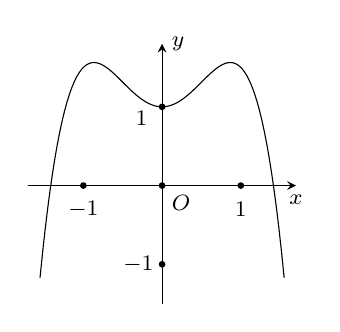
\begin{tikzpicture}
[scale=1, font=\footnotesize, line join=round, line cap=round, >=stealth]
\draw[->] (-1.7,0)--(0,0) node[below right]{$O$}--(1.7,0) node[below]{$x$};
\draw[->] (0,-1.5) --(0,1.8) node[right]{$y$};
\draw [domain=-1.55:1.55, samples=100] %
plot (\x, {-1*(\x)^4+(1.5)*(\x)^2+1});
\draw[fill] (0,0) circle (1pt);
\foreach \x/\g in {-1/-90,1/-90} 
\draw[fill] (\x,0) circle(1pt)node [shift={(\g:.3)}] {$\x$};
\foreach \y/\g in {-1/180,1/210} 
\draw[fill] (0,\y) circle(1pt)node [shift={(\g:.3)}] {$\y$};
\end{tikzpicture}}
\loigiai{
Dựa vào đồ thị, hàm số tương ứng là hàm trùng phương có hệ số $a$ của $x^4$ âm.
}
\end{ex}
\begin{ex}%[Đề thi giữa HKI trường THPT Lý Thường Kiệt, Bình Thuận 2020]%[Trần Hòa, dự án 12-EX-3-2021]%[2H1Y2-2]
Khối lập phương là khối đa diện đều loại nào sau đây?
\choice
{$\{3;4\}$}
{$\{3;5\}$}
{$\{4;4\}$}
{\True $\{4;3\}$}
\loigiai{
Khối lập phương là khối đa diện đều loại $\{4;3\}$.
}
\end{ex}
\begin{ex}%[Đề thi giữa HKI trường THPT Lý Thường Kiệt, Bình Thuận 2020]%[Trần Hòa, dự án 12-EX-3-2021]%[2D1Y1-2]
Cho hàm số $f(x)$ có bảng biến thiên như hình.
\begin{center}
    
\begin{tikzpicture}
\tkzTabInit[nocadre=false,lgt=1,espcl=2.5,deltacl=0.6]%[nocadre=true\fasle(không\có) kẻ viền bảng ,
%lgt=1,espcl=2]:Độ rộng cột thứ nhât, các cột tiếp theo
{$x$ /.7,$y'$ /.7,$y$ /2}{$-\infty$,$-1$,$0$,$1$,$+\infty$}
%số dòng của x(1), y'(1), y(2), các giá trị điền ở dòng
\tkzTabLine{,+,$0$,-,$0$,+,$0$,-,}%điền dấu, giá trị y'
\tkzTabVar{-/$-\infty$ ,+/$3$,-/$-2$,+/$3$,-/$-\infty$} %-/ là giá trị ở dưới thấp
\end{tikzpicture}
\end{center}
 Hàm số $f(x)$ đồng biến trên khoảng nào sau đây?
\choice
{$(1;+\infty)$}
{$(-1;0)$}
{$(-\infty;3)$}
{\True $(0;1)$}
\loigiai{
Dựa vào bảng biến thiên, hàm số $f(x)$ đồng biến trên khoảng $(0;1)$.
}
\end{ex}
\begin{ex}%[Đề thi giữa HKI trường THPT Lý Thường Kiệt, Bình Thuận 2020]%[Trần Hòa, dự án 12-EX-3-2021]%[2H1Y1-2]
Hình bát diện đều có mấy đỉnh?
\choice
{$4$}
{\True $6$}
{$24$}
{$8$}
\loigiai{
Hình bát diện đều có $6$ đỉnh.
}
\end{ex}
\begin{ex}%[Đề thi giữa HKI trường THPT Lý Thường Kiệt, Bình Thuận 2020]%[Trần Hòa, dự án 12-EX-3-2021]%[2H1Y3-2]
Tính thể tích khối lăng trụ có chiều cao bằng $a$ và diện tích đáy bằng $100a^2$.
\choice
{$100a^2+a$}
{$\dfrac{100a^3}{3}$}
{$50a^3$}
{\True $100a^3$}
\loigiai{
Thể tích khối lăng trụ là $V=hS=100a^3$.
}
\end{ex}
\begin{ex}%[Đề thi giữa HKI trường THPT Lý Thường Kiệt, Bình Thuận 2020]%[Trần Hòa, dự án 12-EX-3-2021]%[2H1Y3-2]
Tính thể tích của khối hộp chữ nhật có chiều dài, chiều rộng và chiều cao lần lượt là $2a$, $a$, $3a$.
\choice
{$2a^2+3a$}
{\True $6a^3$}
{$6a$}
{$18a^2$}
\loigiai{
Thể tích khối hộp chữ nhật là $V=2a\cdot a\cdot 3a=6a^3$.
}
\end{ex}
\begin{ex}%[Đề thi giữa HKI trường THPT Lý Thường Kiệt, Bình Thuận 2020]%[Trần Hòa, dự án 12-EX-3-2021]%[2D1Y4-1]
Đồ thị hàm số $y=\dfrac{2x}{x-3}$ có đường tiệm cận đứng là
\choice
{$x=0$}
{$y=3$}
{\True $x=3$}
{$y=2$}
\loigiai{
Tập xác định $\mathscr{D}=\mathbb{R}\setminus\{3\}$.\\
$\lim\limits_{x\to 3^+}\dfrac{2x}{x-3}=+\infty$.\\
Vậy $x=3$ là đường tiệm cận đứng của đồ thị hàm số.
}
\end{ex}
\begin{ex}%[Đề thi giữa HKI trường THPT Lý Thường Kiệt, Bình Thuận 2020]%[Trần Hòa, dự án 12-EX-3-2021]%[2D1Y5-7]
Tọa độ giao điểm của đồ thị hàm số $y=-x^3+2x^2-1$ với trục tung là
\choice
{\True $(0;-1)$}
{$(1;0)$}
{$(-1;0)$}
{$(0;1)$}
\loigiai{
Khi $x=0\Rightarrow y=-1$, nên đồ thị cắt trục tung tại điểm $(0;-1)$.
}
\end{ex}
\begin{ex}%[Đề thi giữa HKI trường THPT Lý Thường Kiệt, Bình Thuận 2020]%[Trần Hòa, dự án 12-EX-3-2021]%[2D1Y1-2] 
\immini{Cho hàm số $f(x)$ xác định trên $\mathbb{R}$ và có đồ thị như hình vẽ bên. Mệnh đề nào dưới đây đúng?
\choice
{\True Hàm số $f(x)$ nghịch biến trên khoảng $(-1;0)$}
{Hàm số $f(x)$ đồng biến trên khoảng $(-2;+\infty)$}
{Hàm số $f(x)$ nghịch biến trên khoảng $(0;2)$}
{Hàm số $f(x)$ đồng biến trên khoảng $(-2;0)$}}{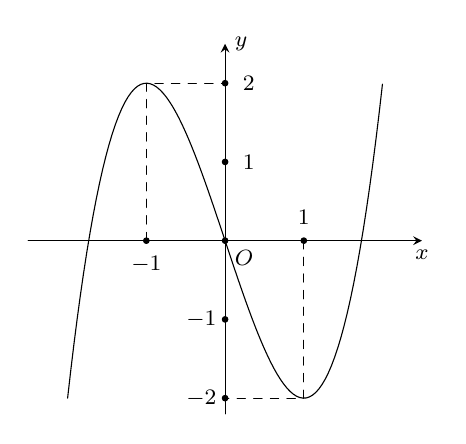
\begin{tikzpicture}
[scale=1, font=\footnotesize, line join=round, line cap=round, >=stealth]
\draw[->] (-2.5,0)--(0,0) node[below right]{$O$}--(2.5,0) node[below]{$x$};
\draw[->] (0,-2.2) --(0,2.5) node[right]{$y$};
\draw [domain=-2:2, samples=100] %
plot (\x, {(\x)^3-3*(\x)});
\draw[fill] (0,0) circle (1pt);
\foreach \x/\g in {-1/-90,1/90} 
\draw[fill] (\x,0) circle(1pt)node [shift={(\g:.3)}] {$\x$};
\foreach \y/\g in {-1/180,1/0,2/0,-2/-180} 
\draw[fill] (0,\y) circle(1pt)node [shift={(\g:.3)}] {$\y$};
\draw[dashed] (-1,0)--(-1,2)--(0,2);
\draw[dashed] (1,0)--(1,-2)--(0,-2);
\end{tikzpicture}}
\loigiai{
Dựa vào đồ thị, hàm số nghịch biến trên khoảng $(-1;0)$.
}
\end{ex}
\begin{ex}%[Đề thi giữa HKI trường THPT Lý Thường Kiệt, Bình Thuận 2020]%[Trần Hòa, dự án 12-EX-3-2021]%[2D1Y2-1]
Cho hàm số $f(x)$ liên tục trên $\mathbb{R}$ và có $f'(x)=x^3+x$. Số điểm cực trị của hàm số $f(x)$ là
\choice
{$4$}
{\True $1$}
{$2$}
{$3$}
\loigiai{
Có $f'(x)=x(x^2+1)$ suy ra $f'(x)=0$ có duy nhất nghiệm $x=0$ và $f'(x)$ đổi dấu qua nghiệm nên hàm số $f(x)$ có $1$ điểm cực trị.
}
\end{ex}
\begin{ex}%[Đề thi giữa HKI trường THPT Lý Thường Kiệt, Bình Thuận 2020]%[Trần Hòa, dự án 12-EX-3-2021]%[2D1B1-1]
Hàm số nào sau đây nghịch biến trên $\mathbb{R}$?
\choice
{$y=-x^4-2x^2+1$}
{$y=-x^3+3x-2018$}
{$y=\dfrac{x-1}{3x-4}$}
{\True $y=-x^3-2x+1$}
\loigiai{
Hàm số $y=-x^3-2x+1$ có $y'=-3x^2-2<0\,\forall x\in\mathbb{R}$ nên hàm số nghịch biến trên $\mathbb{R}$.
}
\end{ex}
\begin{ex}%[Đề thi giữa HKI trường THPT Lý Thường Kiệt, Bình Thuận 2020]%[Trần Hòa, dự án 12-EX-3-2021]%[2H1B3-2] 
\immini{Cho hình tứ diện $ABCD$ có $AB$, $AC$, $AD$ đôi một vuông góc. $AB=4a$, $AC=6a$, $AD=2a$. Gọi $M$ là trung điểm cạnh $AC$. Tính thể tích khối chóp $B.CDM$.
\choice
{$24a^3$}
{$8a^3$}
{$12a^3$}
{\True $4a^3$}}{\begin{tikzpicture}[scale=1, font=\footnotesize, line join=round, line cap=round]
\tkzDefPoints{0/0/A, 4/0/x, 0/3/y}
\coordinate (B) at ($(A)+(y)$);
\coordinate (D) at ($(A)+(x)$);
\coordinate (C) at ($(A)+(3,-2)$);
\coordinate (M) at ($(A)!0.5!(C)$);
\draw (A)--(B)--(C)--(D)--(B);
\draw (A)--(C);
\draw[dashed] (A)--(D)--(M);
\foreach \p/\g in {A/180,B/90,C/-45,D/30,M/-90} \draw[fill] (\p) circle(1pt)node [shift={(\g:.3)}] {$\p$};
\end{tikzpicture}}
\loigiai{
Thể tích khối chóp $B.ACD$ là $V=\dfrac{1}{6}AB\cdot AC\cdot AC=\dfrac{1}{6}4a\cdot 6a\cdot 2a=8a^3$.\\
Vì $M$ là trung điểm $AC$ nên $S_{CDM}=\dfrac{1}{2}S_{ACD}$ nên $V_{B.CDM}=\dfrac{1}{2}V_{B.ACD}=4a^3$.
}
\end{ex}
\begin{ex}%[Đề thi giữa HKI trường THPT Lý Thường Kiệt, Bình Thuận 2020]%[Trần Hòa, dự án 12-EX-3-2021]%[2H1B3-2] 
\immini{Cho khối hộp chữ nhật $ABCD.A'B'C'D'$ có $AA'=a$, $AB=4a$, $BC=3a$. Gọi $O$ là trung điểm đường chéo  $BD'$. Tính thể tích khối chóp $O.BCC'B'$.
\choice
{\True $2a^3$}
{$a^3$}
{$3a^3$}
{$6a^3$}}{\begin{tikzpicture}[scale=1,font=\footnotesize,line join = round, line cap = round, >= stealth]
\coordinate (A) at (0,0);
\def\x{4}
\def\y{2}
\def\z{3}
\def\g{30}% goc hbh đáy
\def\n{90} %goc nghiêng
\coordinate (B) at ($(A)+(\x,0)$);
\coordinate (C) at ($(B)+(\g:\y)$);
\coordinate (D) at ($(A)+(C)-(B)$);
\coordinate (A') at ($(A)+(\n:\z)$);
\coordinate (B') at ($(B)+(\n:\z)$);
\coordinate (C') at ($(C)+(\n:\z)$);
\coordinate (D') at ($(D)+(\n:\z)$);
\coordinate (O) at ($(D')!0.5!(B)$);
\draw (A)--(B)--(B')--(A')--cycle;
\draw (A')--(D')--(C')--(B') (B)--(C)--(C');
\draw[dashed] (A)--(D)--(D') (D)--(C) (B)--(D');
\foreach \p/\g in {A/-90,B/-90,C/-45,D/-90,A'/180,B'/90,C'/90,D'/90,O/-130} \draw[fill] (\p) circle(1pt) node [shift={(\g:.3)}] {$\p$};
\end{tikzpicture}}
\loigiai{
\immini{Gọi $H$ là trung điểm $BC'$ ta có $V_{O.BCC'B'}=\dfrac{1}{3}OH\cdot S_{BCC'B'}=\dfrac{1}{6}AB\cdot BC\cdot BB'=2a^3$.}{\begin{tikzpicture}[scale=1,font=\footnotesize,line join = round, line cap = round, >= stealth]
\coordinate (A) at (0,0);
\def\x{4}
\def\y{2}
\def\z{3}
\def\g{30}% goc hbh đáy
\def\n{90} %goc nghiêng
\coordinate (B) at ($(A)+(\x,0)$);
\coordinate (C) at ($(B)+(\g:\y)$);
\coordinate (D) at ($(A)+(C)-(B)$);
\coordinate (A') at ($(A)+(\n:\z)$);
\coordinate (B') at ($(B)+(\n:\z)$);
\coordinate (C') at ($(C)+(\n:\z)$);
\coordinate (D') at ($(D)+(\n:\z)$);
\coordinate (O) at ($(D')!0.5!(B)$);
\coordinate (H) at ($(B)!0.5!(C')$);
\draw (B)--(C');
\draw (A)--(B)--(B')--(A')--cycle;
\draw (A')--(D')--(C')--(B') (B)--(C)--(C');
\draw[dashed] (A)--(D)--(D') (D)--(C) (B)--(D') (O)--(H);
\foreach \p/\g in {A/-90,B/-90,C/-45,D/-90,A'/180,B'/90,C'/90,D'/90,O/-130,H/0} \draw[fill] (\p) circle(1pt) node [shift={(\g:.3)}] {$\p$};
\end{tikzpicture}}
}
\end{ex}
\begin{ex}%[Đề thi giữa HKI trường THPT Lý Thường Kiệt, Bình Thuận 2020]%[Trần Hòa, dự án 12-EX-3-2021]%[2H1Y1-2] 
Cho hình chóp có tổng số cạnh bên và cạnh đáy bằng $10$. Số mặt bên của hình chóp đó là
\choice
{$6$}
{\True $5$}
{$10$}
{$11$}
\loigiai{
Hình chóp luôn có số cạnh bên bằng số cạnh đáy và bằng số mặt bên. Vậy theo bài ra hình chóp có $5$ cạnh bên và $5$ cạnh đáy nên số mặt bên là $5$.
}
\end{ex}
\begin{ex}%[Đề thi giữa HKI trường THPT Lý Thường Kiệt, Bình Thuận 2020]%[Trần Hòa, dự án 12-EX-3-2021]%[2H1Y2-2]
Trong bốn hình gồm hình chóp tam giác đều, hình chóp tứ giác đều, hình lăng trụ đều và hình bát diện đều. Hỏi có mấy hình là đa diện đều?
\choice
{$3$}
{$4$}
{$2$}
{\True $1$}
\loigiai{
Có $1$ hình đa diện đều là hình bát diện đều.
}
\end{ex}
%%%cau21
\begin{ex}%[Đề thi giữa HKI trường THPT Lý Thường Kiệt, Bình Thuận 2020]%[Tran Tony, dự án 12-EX-3-2021]%[2D1Y1-1]
	Giá trị cực tiểu của hàm số $y=x^3-6x^2+7$ là
	\choice
	{\True $-25$}
	{$12$}
	{$9$}
	{$2$}
	\loigiai{
	Ta có $y'=3x^2-12x$, $y'=0\Leftrightarrow \hoac{&x=0\\&x=4.}$\\
	Bảng biến thiên
	\begin{center}
	
\begin{tikzpicture}
	\tkzTabInit[nocadre=false,lgt=1.2,espcl=2.5,deltacl=0.6]
	{$x$ /0.6, $y'$ /0.6, $y$ /2}
	{$-\infty$,$0$,$4$,$+\infty$}
	\tkzTabLine{ ,+,$0$,-,$0$,+, }
	\tkzTabVar{-/$-\infty$,+/$7$,-/$-25$,+/$+\infty$}
	\end{tikzpicture}
	\end{center}
	Từ bảng biến thiên suy ra giá trị cực tiểu của hàm số là $-25$.
	}
\end{ex}
\begin{ex}%[Đề thi giữa HKI trường THPT Lý Thường Kiệt, Bình Thuận 2020]%[Tran Tony, dự án 12-EX-3-2021]%[2H1B3-4]
	\immini{
		Cho tứ diện $ABCD$ có thể tích bằng $2 \sqrt{3} a^3$, tam giác $ABC$ là tam giác đều, $AB =2a$. Tính khoảng cách từ $D$ đến $(ABC)$.
		\choice
		{\True $6a$}
		{$2a$}
		{$\dfrac{2a}{3}$}
		{ $24a$}
	}
	{
		
	}
	
	\loigiai{
		Ta có $S_{\triangle ABC} = \dfrac{(2a)^2\sqrt{3}}{4} = a^2\sqrt{3} $.\\
		$V_{ABCD}=\dfrac{1}{3}S_{\triangle ABC} \cdot \mathrm{d} \left(D, (ABC) \right) \Rightarrow \mathrm{d} \left(D, (ABC) \right)=\dfrac{3V}{S_{\triangle ABC}}=\dfrac{3\cdot 2 \sqrt{3} a^3 }{a^2\sqrt{3}} =6a$.
	}
\end{ex}
\begin{ex}%[Đề thi giữa HKI trường THPT Lý Thường Kiệt, Bình Thuận 2020]%[Tran Tony, dự án 12-EX-3-2021]%[2D1B5-4]
	Số giao điểm của đồ thị hàm số $y = x^3+3x^2$ và đồ thị hàm số $y = 3x^2+3x$ là
	\choice
	{ $1$}
	{\True $3$}
	{$2$}
	{ $0$}
	\loigiai{
		Phương trình hoành độ giao điểm
		$$x^3+3x^2=3x^2+3x \Leftrightarrow x^3 -3x=0 \Leftrightarrow \hoac{&x=0\\&x=\sqrt{3}\\&x=-\sqrt{3}.}$$
		Vậy hai đồ thị đã cho có $3$ giao điểm.
	}
\end{ex}
\begin{ex}%[Đề thi giữa HKI trường THPT Lý Thường Kiệt, Bình Thuận 2020]%[Tran Tony, dự án 12-EX-3-2021]%[2D1B3-1]
	Giá trị nhỏ nhất của hàm số $f(x)=x^3+3x^2$ trên đoạn $[-4; -1]$ bằng
	\choice
	{\True $f(-4)$}
	{ $f(-3)$}
	{$f(-1)$}
	{ $f(-2)$}
	\loigiai{
		Ta có $f'(x)=3x^2+6x$ và $f'(x)=0 \Leftrightarrow \hoac{&x=0 \notin [-4; -1]\\&x=-2 \in [-4; -1].}$\\
		$f(-4)=-16$, $f(-1)=2$, $f(-2)= 4$.\\
		Vậy $\min\limits_{[-4; -1]} f(x)=f(-4)$.
	}
\end{ex}
\begin{ex}%[Đề thi giữa HKI trường THPT Lý Thường Kiệt, Bình Thuận 2020]%[Tran Tony, dự án 12-EX-3-2021]%[2D1B1-3]
	Tìm số giá trị nguyên của $m$ thỏa mãn hàm số $y = \dfrac{mx-1}{x-m}$ đồng biến trên mỗi khoảng xác định của nó.
	\choice
	{ $3$}
	{ $0$}
	{$2$}
	{ \True $1$}
	\loigiai{
		Tập xác định: $\mathscr{D}=\mathbb{R}\setminus\{m\}$.\\
		Ta có $y'=\dfrac{-m^2+1}{(x-m)^2}$.\\
		Hàm số đồng biến trên mỗi khoảng xác định của nó $\Leftrightarrow -m^2+1 >0 \Leftrightarrow -1 <m<1$.\\
		Vì $m$ nguyên nên $m=0$.\\
		Vậy có $1$ giá trị $m$ nguyên thỏa mãn yêu cầu bài toán.
	}
\end{ex}
\begin{ex}%[Đề thi giữa HKI trường THPT Lý Thường Kiệt, Bình Thuận 2020]%[Tran Tony, dự án 12-EX-3-2021]%[2D1B5-3]
	\immini{
		Cho hàm số $y =f(x)$ xác định trên $\mathbb{R}$ và có đồ thị như hình vẽ bên. Số nghiệm của phương trình $2f(x)=-3$ là
		\choice
		{ $1$}
		{ $0$}
		{\True $3$}
		{ $2$}
	}
	{
		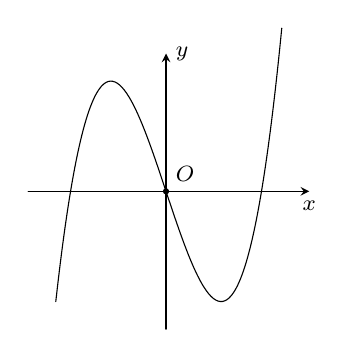
\begin{tikzpicture}[font=\footnotesize,line join=round, line cap=round,>=stealth,scale=0.7]
		\draw[->] (-2.5,0) -- (2.6,0)node[below] {$x$};
		\draw[->] (0,-2.5) -- (0,2.5)node[right] {$y$}; 
		\draw[smooth,samples=100,domain=-2:2.1] plot(\x,{(\x)^3-3*(\x)});
		\draw[fill=black] (0,0) node[above right]{$O$} circle (1.3pt);
		\end{tikzpicture}
	}
	\loigiai{
		Ta có $2f(x)=-3 \Leftrightarrow f(x) = -\dfrac{3}{2}$.\\
		Vì đồ thị hàm số $y = f(x)$ và đường thẳng $y =-\dfrac{3}{2} $ cắt nhau tại $3$ điểm phân biệt nên phương trình đã cho có $3$ nghiệm.
	}
\end{ex}
\begin{ex}%[Đề thi giữa HKI trường THPT Lý Thường Kiệt, Bình Thuận 2020]%[Tran Tony, dự án 12-EX-3-2021]%[2D1B2-3]
	Tìm giá trị thực của tham số $m$ để hàm số $y =\dfrac{1}{3}x^3-mx^2+(m^2-4)x+3$ đạt cực tiểu tại $x = 3$.
	\choice
	{ $m = -1$}
	{ \True $m = 1$}
	{ $m = 5$}
	{ $m = -7$}
	\loigiai{
		Ta có $y'=x^2-2mx+m^2-4$ và $y''= 2x-2m$.\\
		Để hàm số đạt cực tiểu tại $x = 3$ thì trước hết $$y'(3)=0\Leftrightarrow m^2-6m+5=0\Leftrightarrow \hoac{&m=1\\&m=5.}$$
		Với $m=1$, ta có $y''(3)=6-2=4>0$. Hàm số đạt cực tiểu tại $x=3$. Do đó $m=1$ thỏa mãn.\\
		Với $m=5$, ta có $y''(3)=6-10=-4<0$. Hàm số đạt cực đại tại $x=3$. Do đó $m=1$ không thỏa mãn.\\
		Vậy $m = 1$ thỏa mãn yêu cầu yêu cầu bài toán.
	}
\end{ex}
\begin{ex}%[Đề thi giữa HKI trường THPT Lý Thường Kiệt, Bình Thuận 2020]%[Tran Tony, dự án 12-EX-3-2021]%[2H1B3-2]
	\immini{
		Cho khối hộp chữ nhật $ABCD.A'B'C'D'$ có $AB = 3a$, $BC = 4a$, $B'D = a \sqrt{26}$. Tính thể tích khối hộp chữ nhật $ABCD.A'B'C'D'$.
		\choice
		{ $4 \sqrt{26} a^3$}
		{ $4a^3$}
		{ \True $12a^3$}
		{ $12\sqrt{26} a^3$}
	}
	{
		\begin{tikzpicture}[font=\footnotesize,line join=round, line cap=round,>=stealth,scale=0.8]
		\path
		(-1,-1) coordinate (A)
		(2,-1) coordinate (B)
		(3,0) coordinate (C)
		(0,0) coordinate (D)
		(-1,1) coordinate (A')
		(2,1) coordinate (B')
		(3,2) coordinate (C')
		(0,2) coordinate (D')
		;
		\draw (A)--(B)--(C)--(C')--(D')--(A')--(A) (B)--(B')--(A') (B')--(C');
		\draw [dashed] (C)--(D)--(A) (D')--(D)--(B');
		\foreach \x/\g in
		{A/180,B/270,C/0,C'/0,D/170,A'/180,B'/95,D'/170}
		\fill[black](\x) circle (1.1 pt)
		($(\x)+(\g:3mm)$) node{\x};
		\end{tikzpicture}
	}
	\loigiai{
		Xét $\triangle ABC$ vuông tại $B$, có $AC=\sqrt{AB^2+BC^2}=\sqrt{(3a)^2+(4a)^2}=5a$.\\
		Xét $\triangle BB'D'$ vuông tại $B$, có $BB'=\sqrt{B'D^2-BD^2}=\sqrt{\left( a\sqrt{26}\right) ^2-(5a)^2}=a$.\\
		Thể tích khối hộp chữ nhật $ABCD.A'B'C'D'$ là $V = AB \cdot BC \cdot BB' = 3a \cdot 4a \cdot a = 12a^3$.
	}
\end{ex}
\begin{ex}%[Đề thi giữa HKI trường THPT Lý Thường Kiệt, Bình Thuận 2020]%[Tran Tony, dự án 12-EX-3-2021]%[2D1K2-3]
	Tìm tất cả các giá trị của tham số $m$ để hàm số $y = 2 x^4+ (m^2-9)x^2-1$ có $3$ điểm cực trị.
	\choice
	{ $m < 3$}
	{ $-3 \le m \le 3$}
	{ $m < -3$, $m > 3$}
	{ \True $-3 <m< 3$}
	\loigiai{
		Ta có $y' = 8x^3 + 2(m^2-9)x$ và $y'=0 \Leftrightarrow \hoac{& x = 0\\& x^2 = \dfrac{9-m^2}{4}. \qquad(*)} $\\
		Hàm số đã cho có $3$ điểm cực trị phương trình $(*)$ có hai nghiệm phân biệt khác $0$ $$\Leftrightarrow 9 - m^2 > 0 \Leftrightarrow -3 < m < 3.$$ 
	}
\end{ex}
\begin{ex}%[Đề thi giữa HKI trường THPT Lý Thường Kiệt, Bình Thuận 2020]%[Tran Tony, dự án 12-EX-3-2021]%[2D1Y4-1]
	Tiệm cận ngang của đồ thị hàm số $y = \dfrac{\sqrt{x^2+4}}{x-1}$ là
	\choice
	{ $y = -1$}
	{ $y = 1$}
	{\True $y = -1$, $y = 1$}
	{ $x = -1$, $x = 1$}
	\loigiai{
		Ta có  $\lim\limits_{x\rightarrow + \infty} \dfrac{\sqrt{x^2+4}}{x-1} =\lim\limits_{x\rightarrow + \infty} \dfrac{\sqrt{1+\dfrac{4}{x^2}}}{1-\dfrac{1}{x}}= 1 $ và   $\lim\limits_{x\rightarrow - \infty} \dfrac{\sqrt{x^2+4}}{x-1} =\lim\limits_{x\rightarrow - \infty} \dfrac{-\sqrt{1+\dfrac{4}{x^2}}}{1-\dfrac{1}{x}}= -1 $.\\
		Vậy đồ thị hàm số đã cho có hai tiệm cận ngang $y = -1, y = 1$. 
	}
\end{ex}
\begin{ex}%[Đề thi giữa HKI trường THPT Lý Thường Kiệt, Bình Thuận 2020]%[Tran Tony, dự án 12-EX-3-2021]%[2H1Y1-1]
	Hình nào dưới đây không phải là khối đa diện
	\begin{center}
	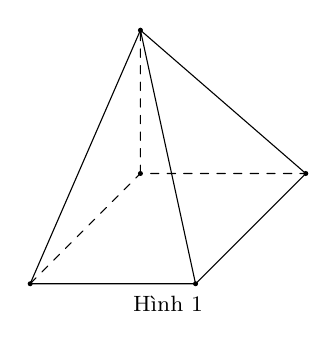
\begin{tikzpicture}[font=\footnotesize,line join=round, line cap=round,>=stealth,scale=0.7]
	\path
	(-2,-2) coordinate (A)
	(1,-2) coordinate (B)
	(3,0) coordinate (C)
	(0,0) coordinate (D)
	(0,2.6) coordinate (S)
	;
	\draw (A)--(B)--(C)--(S)--(A) (S)--(B);
	\draw [dashed] (A)--(D)--(C) (D)--(S);
	\foreach \x in
	{A,B,C,D,S}
	\fill[black](\x) circle (1.3pt);
	\node[below] at (current bounding box.south){Hình 1};
	\end{tikzpicture}
	\hspace{0.4 cm}
	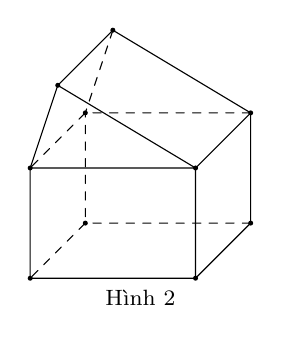
\begin{tikzpicture}[font=\footnotesize,line join=round, line cap=round,>=stealth,scale=0.7]
	\coordinate (A) at (-1,-1);
	\coordinate (B) at (2,-1);
	\coordinate (C) at (3,0);
	\coordinate (D) at (0,0);
	\coordinate (A') at (-1,1);
	\coordinate (B') at (2,1);
	\coordinate (C') at (3,2);
	\coordinate (D') at (0,2);
	\coordinate (E') at (-0.5,2.5);
	\coordinate (G') at (0.5,3.5);
	\draw (A')--(A)--(B)--(C)--(C')--(G')--(E')--(A') (B)--(B')--(A') (E')--(B')--(C');
	\draw [dashed] (C)--(D)--(A) (G')--(D')--(D) (C')--(D')--(A');
	\foreach \x in
	{A,B,C,D,A',B',C',D',E',G'}
	\fill[black](\x) circle (1.3pt);
	\node[below] at (current bounding box.south){Hình 2};
	\end{tikzpicture}
	\hspace{0.4 cm}
	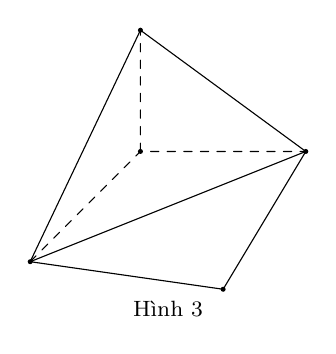
\begin{tikzpicture}[font=\footnotesize,line join=round, line cap=round,>=stealth,scale=0.7]
	\coordinate (A) at (-2,-2);
	\coordinate (B) at (1.5,-2.5);
	\coordinate (C) at (3,0);
	\coordinate (D) at (0,0);	
	\coordinate (S) at (0,2.2);	
	\draw (A)--(B)--(C)--(S)--(A)--(C);	
	\draw [dashed] (A)--(D)--(C) (D)--(S);
	\foreach \x in
	{A,B,C,D,S}
	\fill[black](\x) circle (1.3pt);
	\node[below] at (current bounding box.south){Hình 3};
	\end{tikzpicture}
	\hspace{0.4 cm}
	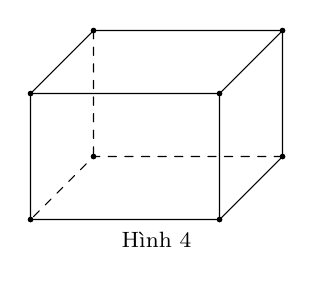
\begin{tikzpicture}[font=\footnotesize,line join=round, line cap=round,>=stealth,scale=0.8]
	\coordinate (A) at (-1,-1);
	\coordinate (B) at (2,-1);
	\coordinate (C) at (3,0);
	\coordinate (D) at (0,0);
	\coordinate (A') at (-1,1);
	\coordinate (B') at (2,1);
	\coordinate (C') at (3,2);
	\coordinate (D') at (0,2);
	\draw (A)--(B)--(C)--(C')--(D')--(A')--(A) (B)--(B')--(A') (B')--(C');
	\draw [dashed] (C)--(D)--(A) (D')--(D);
	\foreach \x in
	{A,B,C,D,A',B',C',D'}
	\fill[black](\x) circle (1.3pt);
	\node[below] at (current bounding box.south){Hình 4};
	\end{tikzpicture}
	\end{center}
	\choice
	{ Hình $1$}
	{ Hình $4$}
	{ \True Hình $3$}
	{ Hình $2$}
	\loigiai{
		Hình $3$ không phải là khối đa diện.
	}
\end{ex}
\begin{ex}%[Đề thi giữa HKI trường THPT Lý Thường Kiệt, Bình Thuận 2020]%[Tran Tony, dự án 12-EX-3-2021]%[2H1B1-2]
	\immini{
		Cho khối lăng trụ đứng $ABC.A'B'C'$ có đáy $ABC$ là các tam giác vuông tại $A$, $AA' = 5a$, $AB = 3a$, $AC=4a$. Tính thể tích khối lăng trụ $ABC.A'B'C'$.
		\choice
		{ $10a^3$}
		{ \True $30a^3$}
		{ $12a^3$}
		{ $60a^3$}
	}
	{
		\begin{tikzpicture}[font=\footnotesize,line join=round, line cap=round,>=stealth,scale=0.7]
		\tkzDefPoints{0/0/A,5/0/C,1.5/-1/B}
		\coordinate (A') at ($(A)+(0,4)$);
		\tkzDefPointsBy[translation = from A to A'](B,C){B'}{C'}
		\tkzDrawPolygon(A,B,C,C',B',A')
		\tkzDrawSegments(A',C' B',B)
		\tkzDrawSegments[dashed](A,C)
		\tkzDrawPoints(A,C,B,A',B',C')
		\tkzLabelPoints[above](B')
		\tkzLabelPoints[below](B)
		\tkzLabelPoints[left](A',A)
		\tkzLabelPoints[right](C',C)
		\end{tikzpicture}
	}
	\loigiai{
		$S_{\triangle ABC} = \dfrac{1}{2} AB \cdot AC =\dfrac{1}{2} 3a \cdot 4a =6a^2$.\\
		Thể tích  khối lăng trụ $ABC.A'B'C'$ là $V = S_{\triangle ABC} \cdot AA'=6a^2 \cdot 5a = 30a^3$.
	}
\end{ex}
\begin{ex}%[Đề thi giữa HKI trường THPT Lý Thường Kiệt, Bình Thuận 2020]%[Tran Tony, dự án 12-EX-3-2021]%[2H1B3-3]
	\immini
	{	Cho khối chóp $S.ABC$. Gọi $M, N$ theo thứ tự là trung điểm các cạnh $SA$, $BC$. Khẳng định nào sau đây \textbf{đúng}?
		\choice
		{ $\dfrac{V_{M.ACN}}{V_{S.ABC}}=\dfrac{1}{2}$}
		{ $\dfrac{V_{M.ACN}}{V_{S.ABC}}=\dfrac{1}{8}$}
		{ $\dfrac{V_{M.ACN}}{V_{S.ABC}}=\dfrac{1}{3}$}
		{ \True $\dfrac{V_{M.ACN}}{V_{S.ABC}}=\dfrac{1}{4}$}
	}
	{
		\begin{tikzpicture}[font=\footnotesize,line join=round, line cap=round,>=stealth,scale=0.7]
		\coordinate[label=left:A] (A) at (-1,0);
		\coordinate[label=right:C] (C) at (3,0);
		\coordinate[label=below:B] (B) at (0,-2);
		\coordinate[label=left:S] (S) at (1,3);
		\coordinate [label=right:N] (N) at ($(B)!.5!(C)$);
		\coordinate [label=left:M] (M) at ($(S)!.5!(A)$);
		\draw (A)--(S)--(C)--(B)--(A) (S)--(B);
		\draw [dashed] (C)--(A)--(N)--(M)--(C);
		\draw (S) circle (1pt) (A) circle (1pt) (B) circle (1pt) (C) circle (1pt) (M) circle (1pt) (N) circle (1pt);
		\end{tikzpicture}
	}
	\loigiai{
		Ta có $S_{\triangle ACN} = \dfrac{1}{2} S_{\triangle ABC}$ (do $N$ là trung điểm $BC$) và hai hình chóp $M.ACN$, $M. ABC$ có cùng chiều cao suy ra $V_{M.ACN} = \dfrac{1}{2} V_{M. ABC}$. \hfill $(1)$\\
		Hai hình chóp $M. ABC$ và $S. ABC$ cùng đáy và tỉ số chiều cao bằng $\dfrac{1}{2}$ nên $V_{M. ABC} = \dfrac{1}{2} V_{S. ABC}$ \hfill $(2)$\\
		Từ $(1)$ và $(2)$, suy ra $V_{M. ACN} = \dfrac{1}{4} V_{S. ABC}$.
	}
\end{ex}
\begin{ex}%[Đề thi giữa HKI trường THPT Lý Thường Kiệt, Bình Thuận 2020]%[Tran Tony, dự án 12-EX-3-2021]%[2D1Y4-1]
	\immini{Cho hàm số $y = f(x)$ có đồ thị như hình vẽ bên. Chọn khẳng định \textbf{sai}.
		\choice
		{ $x = 1$ là tiệm cận đứng của đồ thị hàm số $y = f(x)$}
		{ \True Hàm số $y=f(x)$ nghịch biến trên $\mathbb{R} \setminus \{1\}$}
		{ $y = 1$ là tiệm cận ngang của đồ thị hàm số $y = f(x)$}
		{$\min\limits_{[-2; 0]}f(x)=f(0)$}
	}{
	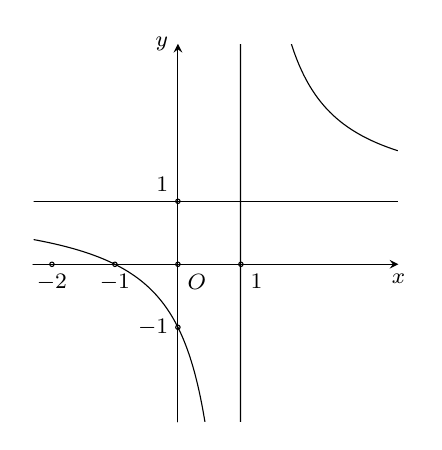
\begin{tikzpicture}[font=\footnotesize,line join=round, line cap=round,>=stealth,scale=0.8]
	\def \xmin{-2.3}
	\def \xmax{3.5}
	\def \ymin{-2.5}
	\def \ymax{3.5}
	\draw[->] (\xmin,0)--(\xmax,0) node[below] {$x$};
	\draw[->] (0,\ymin)--(0,\ymax) node[left] {$y$};
	\draw (-2,0)node[below]{$-2$} circle (1pt) (-1,0)node[below]{$-1$} circle (1pt) (0,0)node[below right]{$O$} circle (1pt) (1,0)node[below right]{$1$} circle (1pt) (0,-1)node[left]{$-1$} circle (1pt) (0,1)node[above left]{$1$} circle (1pt);
	\begin{scope}
	\clip (\xmin+0.01,\ymin+0.01) rectangle (\xmax-0.01,\ymax-0.01);
	\draw[samples=350,domain=\xmin+0.01:\xmax-0.01,smooth,variable=\x] plot (\x,{(\x+1)/(\x-1)});
	\draw[samples=200,domain=\xmin+0.01:\xmax-0.01,smooth,variable=\x] plot (\x,{1});
	\end{scope}
	\end{tikzpicture}
	}
	\loigiai{
	\lq\lq  Hàm số $y=f(x)$ nghịch biến trên $\mathbb{R} \setminus \{1\}$\rq\rq\, là khẳng định \textbf{sai}. Khẳng định đúng tương ứng là \lq\lq  Hàm số $y=f(x)$ nghịch biến trên $(- \infty; 1)$ và $(1; +\infty)$\rq\rq.
	}
\end{ex}
\begin{ex}%[Đề thi giữa HKI trường THPT Lý Thường Kiệt, Bình Thuận 2020]%[Tran Tony, dự án 12-EX-3-2021]%[2D1B4-1]
	Số tiệm cận của đồ thị hàm số $y = \dfrac{x^2-5x+4}{x^2 -1}$ là
	\choice
	{ $1$}
	{ $0$}
	{ $3$}
	{ \True $2$}
	\loigiai{
		$\lim\limits_{x\rightarrow \pm \infty} \dfrac{x^2-5x+4}{x^2 -1} =\lim\limits_{x\rightarrow \pm \infty} \dfrac{1-\dfrac{5}{x}+\dfrac{4}{x^2}}{1 -\dfrac{1}{x^2}}=1$.\\
		Đồ thị hàm số có tiệm cận ngang $y =1$.\\
		$\lim\limits_{x\rightarrow  (-1)^{+}} \dfrac{x^2-5x+4}{x^2 -1} =+ \infty$ và $\lim\limits_{x\rightarrow  (-1)^{-}} \dfrac{x^2-5x+4}{x^2 -1} =- \infty$.\\
		Đồ thị hàm số có tiệm cận đứng $x = -1$.\\
		$\lim\limits_{x\rightarrow  1} \dfrac{x^2-5x+4}{x^2 -1} =\lim\limits_{x\rightarrow  1} \dfrac{x-4}{x +1} =-\dfrac{3}{2}$ nên $x = 1$ không phải tiệm cận đứng của đồ thị hàm số.\\
		Vậy đồ thị hàm số đã cho có $2$ tiệm cận.	
	}
\end{ex}
\begin{ex}%[Đề thi giữa HKI trường THPT Lý Thường Kiệt, Bình Thuận 2020]%[Tran Tony, dự án 12-EX-3-2021]%[2H1K3-5]
	\immini{
	Các kích thước của một bể bơi được cho trên hình vẽ (đo theo mặt trong của bể chứa). Hãy tính xem bể chứa bao nhiêu mét khối nước khi nó đầy ắp nước?
	\choice
	{ $640$ m$^3$}
	{ $600$ m$^3$}
	{ $500$ m$^3$}
	{ \True $570$ m$^3$}
	}{
	\begin{tikzpicture}[scale=0.6,font=\footnotesize,line join = round, line cap = round, >= stealth]
		\path
		(0,0) coordinate (A)
		(10,0) coordinate (x)
		(1.5,2) coordinate (y)
		(0,2) coordinate (z);
		\coordinate (B) at ($(A)+(x)$);
		\coordinate (C) at ($(B)+(y)$);
		\coordinate (D) at ($(A)+(y)$);
		\coordinate (E) at ($(B)-(z)$);
		\coordinate (F) at ($(C)-(z)$);
		\coordinate (K) at ($(A)-(z)-(z)$);
		\coordinate (H) at ($(A)-(z)+(4,0)$);
		\draw[fill,color=blue!40](A)--(B)--(C)--(D)--cycle;
		\draw[fill,pattern=bricks,pattern color=red!20](A)--(B)--(E)--(H)--(K)--cycle;
		\draw[fill,rotate =-60,pattern=bricks,pattern color=red!20](B)--(E)--(F)--(C)--cycle;
		\draw[thick](A)--(B)--(C)--(D)--(A);
		\coordinate (I1) at ($(A)!0.5!(D)$);
		\coordinate (I2) at ($(D)!0.5!(C)$);
		\coordinate (I3) at ($(C)!0.5!(F)$);
		\coordinate (I4) at ($(A)!0.5!(K)$);
		\coordinate (H1) at ($(H)-(z)$);
		\coordinate (I5) at ($(K)!0.5!(H1)$);
		\draw[<->]($(A)+(-0.2,0)$)--($(D)+(-0.2,0)$);
		\tkzLabelSegment[sloped](A,D){$10$m}
		\draw[<->]($(D)+(0,0.2)$)--($(C)+(0,0.2)$);
		\tkzLabelSegment[sloped](D,C){$25$m}
		\draw[<->]($(C)+(0.2,0)$)--($(F)+(0.2,0)$);
		\tkzLabelSegment[sloped](C,F){$2$m}
		\draw[<->]($(K)+(-0.2,0)$)--($(A)+(-0.2,0)$);
		\tkzLabelSegment[sloped](K,A){$4$m}
		\draw[<->]($(K)+(0,-0.2)$)--($(H1)+(0,-0.2)$);
		\tkzLabelSegment[sloped](H1,K){$7$m}
		\draw[dashed](H1)--(H);
	\end{tikzpicture}
	}
	\loigiai{
		Chia bể thành hai khối đa diện
		\begin{itemize} 
			\item Khối hộp chữ nhật có chiều dài $25$ m, chiều rộng $10$ m, chiều cao $2$ m. \\
			Thể tích khối hộp chữ nhật là: $V_1 = 25 \cdot 10 \cdot 2 = 500$ m$^3$.
			\item Khối lăng trụ đứng có chiều cao $10$ m, đáy là tam giác vuông có hai cạnh góc vuông là $2$ m, $7$ m.\\
			Thể tích khối lăng trụ tam giác là: $V_2 = \dfrac{1}{2} \cdot 2 \cdot 7 \cdot 10 = 70$ m$^3$.
		\end{itemize}
		Thể tích phần chứa nước của bể là $V = V_1+ V_2 = 500+70 = 570$ m$^3$.
	} 
\end{ex}
\begin{ex}%[Đề thi giữa HKI trường THPT Lý Thường Kiệt, Bình Thuận 2020]%[Tran Tony, dự án 12-EX-3-2021]%[2D1B5-4]
	Tìm tất cả các giá trị thực của tham số $m$ để phương trình $x^3 -3x^2 +m =0$ có ba nghiệm thực phân biệt.
	\choice
	{\True $0 < m < 4$}
	{ $-4 < m < 0$}
	{ $m > 2$}
	{  $m < -3$}
	\loigiai{
		Ta có $x^3 -3x^2 +m =0 \Leftrightarrow m = -x^3+3x^2$.\\
		Xét hàm số $f(x) =-x^3+3x^2 $.\\
		Ta có $f'(x) = -3x^2+6x$ và $f'(x) = 0 \Leftrightarrow \hoac{& x=0\\&x=2.}$\\
		Bảng biến thiên
		\begin{center}
			
\begin{tikzpicture}\tkzTabInit[nocadre=false,lgt=1.2,espcl=2.5,deltacl=0.6]
			{$x$ /.6, $f’(x)$ /.6, $f(x)$/2}
			{$-\infty$ , $0$ , $2$ , $+\infty$}
			\tkzTabLine { , -, $0$ , + , $0$ , - , }
			\tkzTabVar {+/$+\infty$, -/$ 0 $ ,+/$ 4 $, -/$-\infty$}
			\end{tikzpicture}
		\end{center}
		Phương trình đã cho có $3$ nghiệm phân biệt $\Leftrightarrow$ Đồ thị hàm số $y = -x^3+3x^2$ cắt đường thẳng $y = m$ tại $3$ điểm phân biệt.\\
		Dựa vào bảng biến thiên, $0 < m< 4$ thỏa mãn yêu cầu bài toán.
	}
\end{ex}
\begin{ex}%[Đề thi giữa HKI trường THPT Lý Thường Kiệt, Bình Thuận 2020]%[Tran Tony, dự án 12-EX-3-2021]%[2D1K2-2]
	\immini{Cho hàm số $y=f(x)$ có đạo hàm cấp $2$ trên $\mathbb{R}$ và đồ thị hàm số $y=f''(x)$ là đường cong như hình vẽ bên. Hàm số $y=f(x)$ có tối đa bao nhiêu điểm cực trị?
		\choice
		{ $3$}
		{ $4$}
		{ $1$}
		{ \True $2$}
	}{
	\begin{tikzpicture}[font=\footnotesize,line join=round, line cap=round,>=stealth,scale=0.8]
		\draw[->] (-2.5,0)--(3.5,0) node[above] {$x$};
		\draw[->] (0,-2)--(0,2.5) node[left] {$y$};
		\fill[black] (-2,0)node[below left]{$-2$} circle (1.2pt) (0,0)node[above right]{$O$} circle (1.2pt) (3,0)node[above]{$3$} circle (1.2pt);
		\draw (-2.4,2.5).. controls (-2.3,2) and (-2.2,1) .. (-2,0);
		\draw (-2,0).. controls (-1.5,-2) and (-0.5,-0) .. (0,0);
		\draw (0,0).. controls (1,-0.2) and (1.5,-1) .. (2,-0.9);
		\draw (2,-0.9).. controls (2.5,-0.7) and (2.6,-0.1) .. (3,0);
		\draw (3,0).. controls (3.3,-0.1) and (3.5,-0.5) .. (3.5,-2);
	\end{tikzpicture}
	}
	\loigiai{
	Từ đồ thị hàm số $y=f''(x)$, ta suy ra bảng biến thiên của hàm số $y=f'(x)$
	\begin{center}
	
\begin{tikzpicture}
	\tkzTabInit[nocadre=false,lgt=1.2,espcl=3,deltacl=0.6]
	{$x$/0.7,$f’'(x)$/0.7,$f'(x)$/2}
	{$-\infty$,$-2$,$+\infty$}
	\tkzTabLine{ ,+,$0$,-, }
	\tkzTabVar{-/,+/$f'(-2)$,-/}
	\end{tikzpicture}
	\end{center}
	Từ bảng biến thiên của hàm số $y=f'(x)$, ta thấy đồ thị hàm số $y=f'(x)$ cắt trục hoành tối đa hai tại hai điểm. Suy ra phương trình $f'(x)=0$ có tối đa hai nghiệm và do đó $f'(x)$ đổi dấu tối đa hai lần.\\
	Vậy hàm số $y=f(x)$ có tối đa $2$ điểm cực trị.
	}
\end{ex}
\begin{ex}%[Đề thi giữa HKI trường THPT Lý Thường Kiệt, Bình Thuận 2020]%[Tran Tony, dự án 12-EX-3-2021]%[2D1K1-3]
	Tìm tập hợp các giá trị $m$ để hàm số $y =\dfrac{x+1}{x+m}$ đồng biến trên khoảng $\left(- \infty; -5 \right) $.
	\choice
	{ $(1; 5)$}
	{ \True $(1;5]$}
	{ $[1; 5]$}
	{  $\left(1; + \infty \right) $}
	\loigiai{
		Điều kiện: $x\neq -m$.
		Ta có $y'=\dfrac{m-1}{(x+m)^2}$.\\
		Hàm số đã cho đồng biến trên $\left(- \infty; -5 \right) $ $\Leftrightarrow \heva{&m-1>0\\&-m \notin \left(- \infty; -5 \right) } \Leftrightarrow \heva{&m > 1\\& m \le 5}\Leftrightarrow 1<m\leq 5$.\\ 
		Vây tập hợp các giá trị của $m$ thỏa mãn là $(1;5]$.
	}
\end{ex}
\begin{ex}%[Đề thi giữa HKI trường THPT Lý Thường Kiệt, Bình Thuận 2020]%[Tran Tony, dự án 12-EX-3-2021]%[2H1B3-2]
	\immini{
		Cho hình chóp $S.ABC$ có mặt bên $SAB$ là tam giác cân tại đỉnh $S$ và nằm trong mặt phẳng vuông góc với đáy, $SB$ tạo với mặt phẳng đáy một góc $60^ \circ$, $AB = AC = a$, $\widehat{BAC} = 120^\circ$. Tính thể tích khối chóp $S.ABC$.
		\choice
		{ $\dfrac{a^3}{16}$}
		{ $\dfrac{a^3}{4}$}
		{\True $\dfrac{a^3}{8}$}
		{ $\dfrac{3a^3}{8}$}
	}
	{
		\begin{tikzpicture}[font=\footnotesize,line join=round, line cap=round,>=stealth]
		\path
		(0:0) coordinate (A)
		(-2,-1.5) coordinate (B)
		(4,0) coordinate (C)
		(-1,2.5) coordinate (S)
		($(A)!1/2!(B)$) coordinate (H)
		;
		\draw (B)--(C)--(S)--(B);
		\draw [dashed] (C)--(A)--(S)--(H) (A)--(B);
		\draw (0.4,-0.4) node[rotate=25]{$120^\circ$};
		\draw pic[draw, angle radius=3mm]{angle=B--A--C};
		\foreach \x/\g in
		{A/180,B/160,C/270,S/180}
		\fill[black](\x) circle (1.2pt)
		($(\x)+(\g:3mm)$) node{\x};
		\end{tikzpicture}
	}
	\loigiai{
		$S_{\triangle ABC} =\dfrac{1}{2} \cdot a \cdot a \sin 120^\circ = \dfrac{a^2 \sqrt{3}}{4}$.\\
		Góc giữa $SB$ và mặt phẳng $(ABC)$ là $\widehat{SBH} = 60 ^ \circ$.\\
		Xét $\triangle SHB$ có $\tan 60 ^ \circ = \dfrac{SH}{HB} \Leftrightarrow SH = HB\tan 60 ^ \circ= \dfrac{a}{2} \sqrt{3} =\dfrac{a \sqrt{3}}{2}$.\\
		Vậy thể tích khối chóp $S.ABC$ là $V = \dfrac{1}{3}\cdot \dfrac{a \sqrt{3}}{2} \cdot \dfrac{a^2 \sqrt{3}}{4} =\dfrac{a^3}{8}$.
	}
\end{ex}
\begin{ex}%[Đề thi giữa kì 1, THPT Lí Thường Kiệt, Bình Thuận]%[Nguyễn Quang Dũng, dự án 12-EX-3-2021]%[2D1K1-2]
Cho hàm số $f(x)$ có bảng xét dấu $f'(x)$ như sau
\begin{center}

\begin{tikzpicture}[font=\footnotesize, line join=round, line cap=round, >=stealth]
\tkzTabInit[nocadre=false,lgt=1.2,espcl=2.5,deltacl=0.6]{$x$ /0.6,$f’(x)$ /0.6}{$-\infty$,$-3$,$-1$,$1$,$+\infty$}
\tkzTabLine{,-,$0$,+,$0$,-,$0$,+}
\end{tikzpicture}
\end{center}
Hàm số $f(3-2x)$ nghịch biến trên khoảng nào dưới đây?
\choice
{$(-2;1)$}
{\True $(4;+\infty)$}
{$(2;4)$}
{$(1;3)$}
\loigiai{
Xét $g(x)=f(2-3x)$, ta có $g'(x)=-3f'(2-3x)$. \\
Ta có $g'(x)<0\Leftrightarrow -3f'(3-2x)<0\Leftrightarrow f'(3-2x)>0\Leftrightarrow\hoac{&-3<3-2x<-1\\&3-2x>1}\Leftrightarrow\hoac{&-6<-2x<-4\\&-2x>-2}\Leftrightarrow\hoac{&2<x<3\\&x<1.}$\\
Do vậy, trong các khoảng đã cho thì hàm số nghịch biến trên khoảng $(-2;1)$.
}
\end{ex}
\begin{ex}%[Đề thi giữa kì 1, THPT Lí Thường Kiệt, Bình Thuận]%[Nguyễn Quang Dũng, dự án 12-EX-3-2021]%[2D1K3-2]
Cho hàm số $y=\dfrac{x+m}{x-1}$ ($m$ là tham số thực) và $\min\limits_{[2;4]}y=3$. Mệnh đề nào dưới đây đúng?
\choice
{$m<-1$}
{$3<m\le 4$}
{\True $m>4$}
{$1\le m<3$}
\loigiai{
Ta có $y'=\dfrac{(x-1)-(x+m)}{(x-1)^2}=\dfrac{-1-m}{(x-1)^2}$.
\begin{itemize}
\item Với $-1-m=0$, ta có $m=-1$.\\
 Hàm số trở thành $y=\dfrac{x-1}{x-1}=1$, do đó $m=-1$ không thỏa mãn yêu cầu bài toán.
\item Với $-1-m>0\Leftrightarrow m< -1$.\\
Ta có $\min\limits_{[2;4]}=y(2)=3\Leftrightarrow \dfrac{2+m}{2-1}=3\Leftrightarrow m=1$ (không thỏa mãn).
\item Với $-m-1<0\Leftrightarrow m>-1$.\\
 Ta có $\min\limits_{[2;4]}y=y(4)=3\Leftrightarrow \dfrac{4+m}{4-1}=3\Leftrightarrow m=5$ (thỏa mãn).
\end{itemize}
}
\end{ex}
\begin{ex}%[Đề thi giữa kì 1, THPT Lí Thường Kiệt, Bình Thuận]%[Nguyễn Quang Dũng, dự án 12-EX-3-2021]%[2D1B2-2]
\immini{Biết hàm số $y=f(x)$ có đạo hàm liên tục trên $\mathbb{R}$ và có đồ thị $f'(x)$ như hình vẽ bên. Tìm số điểm cực trị của hàm số $f(x)$.
\choice
{$4$}
{$1$}
{\True $3$}
{$2$}}
{\begin{tikzpicture}[scale=0.7,font=\footnotesize, line join=round, line cap=round, >=stealth]
\draw[->](-1,0)--(5,0)node[below]{$x$};
\draw[->](0,-2)--(0,3)node[left]{$y$};
\clip(0,-2)rectangle(5,3);
\draw[domain=0:4,samples=100]plot(\x,{(\x-1)*(\x-1)*(\x-3)+0.5});
\foreach \d/\g in{1/-90,2/90,3/-45}
\draw[fill=black](\d,0)circle(1pt)node[shift={(\g:0.35)}]{$\d$};
\end{tikzpicture}
}
\loigiai{
Từ đồ thị của hàm số $f'(x)$ ta thấy $f'(x)=0$ có $3$ nghiệm phân biệt và đổi dấu khi đi qua $3$ nghiệm này nên hàm số đã cho có $3$ điểm cực trị.
}
\end{ex}
\begin{ex}%[Đề thi giữa kì 1, THPT Lí Thường Kiệt, Bình Thuận]%[Nguyễn Quang Dũng, dự án 12-EX-3-2021]%[2D1G3-4]
Cho hàm số $f(x)=\left|x^2-5x+4\right|+mx$. Có bao nhiêu giá trị nguyên thỏa mãn $\min f(x)>1$?
\choice
{$5$}
{$2$}
{\True $7$}
{$1$}
\loigiai{
Ta có $f(x)=\left|x^2-5x+4\right|+mx=\heva{&x^2-(5-m)x+4,\,\text{nếu}\,\, x\in\left(-\infty;1\right]\cup\left[4;+\infty\right)\\&-x^2+(5+m)x-4,\,\text{nếu}\,\, x\in(1;4).}$
\begin{itemize}
\item \textbf{Trường hợp 1:} $x\in\left(-\infty;1\right]\cup\left[4;+\infty\right)$.\\
\begin{itemize}
\item Nếu $1<\dfrac{5-m}{2}<4\Leftrightarrow -3<m<3$ thì $\min f(x)=\min\left\{f(1);f(4)\right\}$. \\
Do đó $\min f(x)>1\Leftrightarrow \heva{&f(1)>1\\&f(4)>1}\Leftrightarrow\heva{&-1+5+m-4>1\\&-16+4(5+m)-4>1}\Leftrightarrow m>1$.\\
 Kết hợp điều kiện đang xét suy ra $m\in(1;3)$.
 \item Nếu $\dfrac{5-m}{2}\notin \left(1;4\right)\Leftrightarrow m\in(-\infty;-3]\cup[3;+\infty)$.\\
 Khi đó $\min f(x)=f\left(\dfrac{5-m}{2}\right)>1\Leftrightarrow-\dfrac{(5-m)^2-16}{4}>1\Leftrightarrow m^2-10m+13<0\Leftrightarrow m\in\left(5-2\sqrt{3};5+2\sqrt{3}\right)$.\\
 Kết hợp điều kiện đang xét suy ra $m\in\left[3;5+2\sqrt{2}\right)$.
\end{itemize}
Vậy $f(x)>1,\forall x\in\left(-\infty;1\right]\cup[4;+\infty)\Leftrightarrow m\in \left(1;5+2\sqrt{3}\right)$. 
 \item \textbf{Trường hợp 2:} $x\in\left(1;4\right)$.\\
 Ta có $f(x)=-x^2+(5+m)x-4>1,\forall x\in(1;4)\Leftrightarrow \heva{&f(1)>1\\&f(4)>1}\Leftrightarrow\heva{&-1+5+m-4>1\\&-16+4(5+m)-4>1}\Leftrightarrow m>1$.
\end{itemize}
Từ các trường hợp trên suy ra $f(x)>1$ khi và chỉ khi $\heva{&m\in\left(1;5+2\sqrt{3}\right)\\&m>1}\Leftrightarrow m\in\left(1;5+2\sqrt{3}\right)$.\\
Do $m\in\mathbb{Z}\Rightarrow m\in\{2;3;\ldots;8\}$.
}
\end{ex}
\begin{ex}%[Đề thi giữa kì 1, THPT Lí Thường Kiệt, Bình Thuận]%[Nguyễn Quang Dũng, dự án 12-EX-3-2021]%[2D1G3-6]
Để thiết kế một chiếc bể nuôi cá Koi hình hộp chữ nhật không nắp có chiều cao $150$ cm và có thể tích chứa $90$ m$^3$. Biết giá thành để làm mặt bên là $2800000$ đồng/m$^2$ và làm mặt đáy là $4000000$ đồng/m$^2$. Tính chi phí thấp nhất để hoàn thành bể cá.
\choice
{\True $370.132.000$ đồng}
{$480{.}000{.}000$ đồng}
{$305{.}066{.}000$ đồng}
{$130{.}132{.}000$ đồng}
\loigiai{
\immini{
Gọi $a$, $b$ lần lượt là các kích thước của hình chữ nhật đáy tính theo đơn vị m, chiều cao bể là $h=1{,}5$ m.\\
Chi phí làm mặt đáy là $S_1=ab\cdot 4000000$ đồng.\\
Chi phí làm mặt bên là $S_2=2h\left(a+b\right)\cdot 2800000$ đồng.\\
Tổng chi phí là $S=2h\left(a+b\right)\cdot 2800000+ab\cdot 4000000$.\\
Theo giả thiết ta có $V=abh=90$ m$^3$.
}
{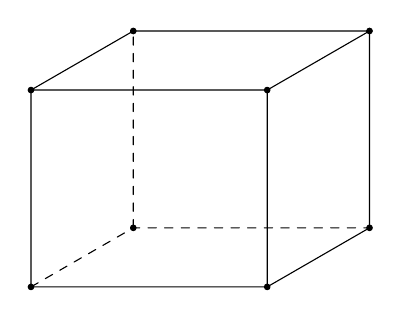
\begin{tikzpicture}[font=\footnotesize, line join=round, line cap=round, >=stealth]
\def\a{3}
\def\h{2.5}
\def\b{0.5*\a}
\def\goc{30}
\path(0,0)coordinate(A)++(\a,0)coordinate(B)++(\goc:\b)coordinate(C)++(180:\a)coordinate(D);
\path[shift={(0,\h)}](0,0)coordinate(A')++(\a,0)coordinate(B')++(\goc:\b)coordinate(C')++(180:\a)coordinate(D');
\draw(A)--(B)--(C)--(C')--(D')--(A')--(B')--(B)(A)--(A')--(B')--(C');
\draw[dashed](A)--(D)--(C)(D)--(D');
\foreach \d in{A,B,C,D,A',B',C',D'}
\draw[fill=black](\d)circle(1pt);
\end{tikzpicture}
}
Suy ra
\begin{eqnarray*}
 S&\ge &4h\sqrt{ab}\cdot 2800000+ab\cdot 4000000\\
 &=&11200000\sqrt{h}\cdot\sqrt{abh}+4000000\cdot\dfrac{V}{h}\\
 &=&11200000\cdot\sqrt{1{,}5}\cdot\sqrt{90}+4000000\cdot 90\cdot\dfrac{1}{1{,}5}\\
 &\approx& 130372000
\end{eqnarray*}
Do vậy chi phí ít nhất là $130{.}132{.}000$ đồng.
}
\end{ex}
\begin{ex}%[Đề thi giữa kì 1, THPT Lí Thường Kiệt, Bình Thuận]%[Nguyễn Quang Dũng, dự án 12-EX-3-2021]%[2D1B4-1]
Cho hàm số $y=f(x)$ xác định trên $\mathbb{R}\setminus\{-1;2\}$, liên tục trên các khoảng xác định và có bảng biến thiên như sau
\begin{center}
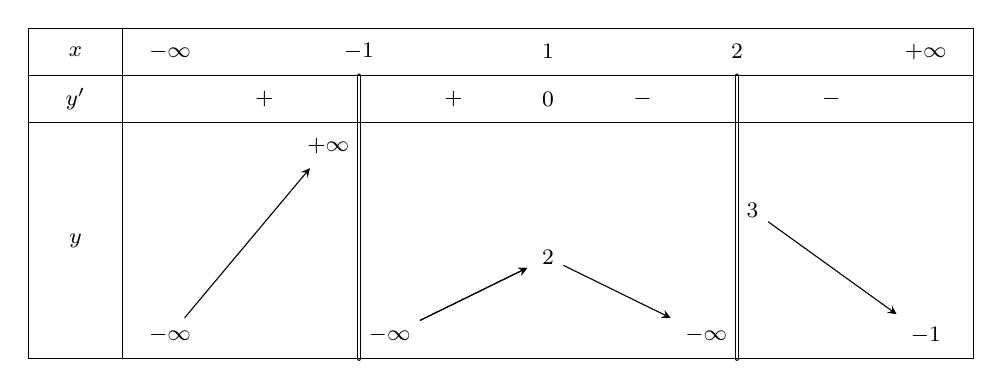
\begin{tikzpicture}[font=\footnotesize, line join=round, line cap=round, >=stealth]
\begin{scope}[yscale=0.6,xscale=1.2,shift={(-0.5,0.5)}]
\draw[double,shift={(0.5,0)}](3,-1)--(3,-7)(7,-1)--(7,-7);
\draw(0,0) rectangle(10,-7)(0,-1)--(10,-1)(1,0)--(1,-7)(0,-2)--(10,-2);
\end{scope}
\begin{scope}[yscale=0.6,xscale=1.2]
\path(0,0) node{$x$}++(1,0)node{$-\infty$}++(2,0)node{$-1$}++(2,0)node{$1$}++(2,0)node{$2$}++(2,0)node{$+\infty$};
\path (0,-1) node{$y'$}++(2,0)node{+}++(2,0)node{$+$}++(1,0)node{$0$}++(1,0)node{$-$}++(2,0)node{$-$};
\path(0,-4)node{$y$}++(1,-2)node(A){$-\infty$}++(2,4)node(B)[left]{$+\infty$}++(0,-4)node(C)[right]{$-\infty$}++(2,2)node[below](D){$2$}++(2,-2)node(E)[left]{$-\infty$}++(0,3)node(F)[below right]{$3$}++(2,-3)node(G){$-1$};
\end{scope}
\begin{scope}[-stealth,shorten >= 2pt]
\draw(A)--(B);
\draw(C)--(D);
\draw(C)--(D);
\draw(D)--(E);
\draw(F)--(G);
\end{scope}
\end{tikzpicture}
\end{center}
Số đường tiệm cận của đồ thị hàm số $y=f(x)$ là
\choice
{$4$}
{\True $3$}
{$5$}
{$6$}
\loigiai{
Từ bảng biến thiên suy ra đồ thị hàm số có các tiệm cận đứng là $x=-1$, $x=2$ và đồ thị hàm số có tiệm cận ngang $y=-1$.\\
Vậy đồ thị hàm số có đúng $3$ tiệm cận.
}
\end{ex}
\begin{ex}%[Đề thi giữa kì 1, THPT Lí Thường Kiệt, Bình Thuận]%[Nguyễn Quang Dũng, dự án 12-EX-3-2021]%[2D1B5-6]
Viết phương trình tiếp tuyến của đồ thị $(H)\colon y=\dfrac{2x-4}{x-3}$ tại $M$ là giao điểm của đồ thị $(H)$ với trục hoành.
\choice
{\True $y=-2x+4$}
{$y=-2x-4$}
{$y=2x$}
{$y=2x-4$}
\loigiai{
Giao điểm của $(H)$ với $Ox$ có tọa độ là $M(2;0)$. Ta có $y'=\dfrac{2(x-3)-(2x-4)}{(x-3)^2}=-\dfrac{2}{(x-3)^2}$.\\
Phương trình của tiếp tuyến của $(H)$ tại $M$ là
\[y=y'(2)(x-2)=-2(x-2)=-2x+4.\]
}
\end{ex}
\begin{ex}%[Đề thi giữa kì 1, THPT Lí Thường Kiệt, Bình Thuận]%[Nguyễn Quang Dũng, dự án 12-EX-3-2021]%[2H1K3-3]
Cho lăng trụ $ABC.A'B'C'$. Gọi $M$ là trung điểm của $BB'$, $N$ là điểm trên cạnh $CC'$ sao cho $CN=3NC'$. Tính tỉ số $\dfrac{V_{A.BMNC}}{V_{ABC.A'B'C'}}$.
\choice
{$\dfrac{5}{24}$}
{$\dfrac{2}{3}$}
{\True $\dfrac{5}{12}$}
{$\dfrac{5}{8}$}
\loigiai{
\immini{
Ta có $V_{A.BB'C'C}=V_{ABC.A'B'C'}-V_{A.A'B'C'}=\dfrac{2}{3}V_{ABC.A'B'C'}$.\\
Mặt khác $S_{BMNC}=\left(\dfrac{1}{2}+\dfrac{3}{4}\right)BB'\cdot\dfrac{1}{2}\cdot\mathrm{d}\left(C,BB'\right)=\dfrac{5}{8}S_{BB'C'C}$.\\
Suy ra $V_{A.BMNC}=\dfrac{2}{3}\cdot\dfrac{5}{8}V_{ABC.A'B'C'}\Rightarrow \dfrac{V_{A.BMNC}}{V_{ABC.A'B'C'}}=\dfrac{5}{12}$.
}
{\begin{tikzpicture}[font=\footnotesize, line join=round, line cap=round, >=stealth]
\def\a{3}
\def\h{2}
\def\b{0.5*\a}
\def\goc{-30}
\path(0,0)coordinate(A)++(\a,0)coordinate(B)(A)++(\goc:\b)coordinate(C);
\path[shift={(0,\h)}](0,0)coordinate(A')++(\a,0)coordinate(B')(A')++(\goc:\b)coordinate(C');
\path($(B)!0.5!(B')$)coordinate(M)($(C)!3/4!(C')$)coordinate(N);
\draw(A)--(C)--(B)(A')--(B')--(C')--(A')(A)--(A')(C)--(C')(B)--(B')(A)--(N)--(M);
\draw[dashed](A)--(B)(A)--(M);
\foreach \d/\g in{M/0,N/180,A/180,C/-90,B/0,A'/90,C'/90,B'/90}
\draw[fill=black](\d)circle(1pt)node[shift={(\g:0.35)}]{$\d$};
\end{tikzpicture}
}
}
\end{ex}
\begin{ex}%[Đề thi giữa kì 1, THPT Lí Thường Kiệt, Bình Thuận]%[Nguyễn Quang Dũng, dự án 12-EX-3-2021]%[2D1K5-1]
\immini{Cho hàm số $y=ax^3+bx^2+cx+d$ có đồ thị như hình vẽ bên. Mệnh đề nào sau đây \textbf{sai}?
\choice
{$bd<0$}
{\True $bc<0$}
{$ac<0$}
{$ab<0$}}
{
\begin{tikzpicture}[font=\footnotesize, line join=round, line cap=round, >=stealth]
\draw[->](-2,0)--(3,0)node[below]{$x$};
\draw[->](0,-1.5)--(0,2.5)node[left]{$y$};
\clip(-2,-1.5)rectangle(3,2.5);
\begin{scope}[yscale=0.2,xscale=0.5]
\draw[domain=-3:4,samples=100]plot(\x,{(\x+2)*((\x)^2-(11/3)*(\x)+2)});
\foreach \d/\g in{-2/135,1/90,2/90,3/-45}
\draw[fill=black](\d,0)circle(1pt)node[shift={(\g:0.35)}]{$\d$};
\draw[dashed](2,0)--(2,{4*(4-22/3+2)});
\end{scope}
\end{tikzpicture}
}
\loigiai{
Ta có $y'=3ax^2+2bx+c$
Từ  hình dáng đồ thị suy ra $a>0$, $y(0)=d>0$.\\
Hàm số có hai điểm cực trị $-2<x_1<x_2=2$, $x_1+x_2=-\dfrac{2b}{3a}>0\Rightarrow b<0$. Mặt khác $x_1x_2=\dfrac{c}{3a}<0$ nên $c<0$.\\
Suy ra $bd<0$, $bc>0$, $ac<0$ và $ab<0$. Khẳng định sai là $bc<0$.
}
\end{ex}
\begin{ex}%[Đề thi giữa kì 1, THPT Lí Thường Kiệt, Bình Thuận]%[Nguyễn Quang Dũng, dự án 12-EX-3-2021]%[2D1K3-1]
\immini{Cho hàm số $y=f(x)$ liên tục trên đoạn $\left[\dfrac{1}{4};\dfrac{7}{3}\right]$ có đồ thị hàm số $y=f'(x)$ như hình vẽ bên. Hàm số đạt giá trị lớn nhất trên đoạn $\left[\dfrac{1}{2};3\right]$ tại điểm $x_0$ nào dưới đây?
\choice
{\True $x_0=\dfrac{1}{2}$}
{$x_0=1$}
{$x_0=3$}
{$x_0=0$}}
{
\begin{tikzpicture}[scale=0.7,font=\footnotesize, line join=round, line cap=round, >=stealth]
\draw[->](-1,0)--(5,0)node[below]{$x$};
\draw[->](0,-2)--(0,3)node[left]{$y$};
\clip(0,-2)rectangle(5,3);
\draw[domain=0:4,samples=100]plot(\x,{(\x-1)*(\x-1)*(\x-3)});
\foreach \d/\g in{1/90,2/90,3/-45}
\draw[fill=black](\d,0)circle(1pt)node[shift={(\g:0.35)}]{$\d$};
\end{tikzpicture}
}
\loigiai{
Bảng biến thiên của hàm số trên đoạn $\left[\dfrac{1}{2};3\right]$ như hình dưới đây.
\begin{center}
\begin{tikzpicture}[font=\footnotesize, line join=round, line cap=round, >=stealth]
\tkzTabInit[nocadre=false,lgt=1.2,espcl=2.5,deltacl=0.6]{$x$ /1,$f’(x)$ /0.6,$f(x)$ /2}{$\dfrac{1}{2}$,$1$,$3$}
\tkzTabLine{,$-$,$0$,$-$,}
\path(N12)node[below](A){$f\left(\dfrac{1}{2}\right)$}(N33)node[above](B){$f(3)$};
\draw[-stealth](A)--(B);
\end{tikzpicture}
\end{center}
Từ bảng biến thiên suy ra trên đoạn $\left[\dfrac{1}{2};3\right]$ hàm số đạt giá trị lớn nhất tại $x=\dfrac{1}{2}$.
}
\end{ex}
\Closesolutionfile{ans}
\begin{indapan}{10}
	{ans/ans-2-GHK1-26-LyThuongKiet-BinhThuan-21}
\end{indapan}
